\documentclass[conference]{IEEEtran}
\IEEEoverridecommandlockouts
\usepackage{amsmath,amssymb,mathtools}
\usepackage{graphicx}
\usepackage{booktabs}
\usepackage{multirow}
\usepackage{array}
\usepackage{float}
\usepackage{hyperref}
\usepackage{xcolor}
\usepackage{amsthm}
\usepackage[caption=false,font=footnotesize]{subfig}

\hypersetup{colorlinks=true,linkcolor=black,citecolor=black,urlcolor=black}

\theoremstyle{plain}
\newtheorem{theorem}{Theorem}
\newtheorem{lemma}{Lemma}
\newtheorem{proposition}{Proposition}
\newtheorem{corollary}{Corollary}

\theoremstyle{definition}
\newtheorem{definition}{Definition}
\newtheorem{assumption}{Assumption}
\newtheorem{remark}{Remark}

\title{A Rigorous CG-Corrected Residual Certificate for Error Certification of Learned Elliptic PDE Solvers}

\author{\IEEEauthorblockN{certno}\IEEEauthorblockA{Error-Certified Neural Operators Project\\\url{https://github.com/emmettv1191/certno-phd-research}}}

\begin{document}
\maketitle

\begin{abstract}
We present a rigorous a posteriori error certification framework for learned surrogates of elliptic partial differential equations. For the discrete symmetric positive definite (SPD) system $A_h u_h = f$ arising from $-\nabla\cdot(a\nabla u)=f$, any candidate $\hat{u}$ satisfies the exact residual identity $e = u_h - \hat{u} = A_h^{-1}(f - A_h \hat{u}) = A_h^{-1}r$. While the global bound $\|e\|_2 \le \|r\|_2/\lambda_{\min}(A_h)$ is mathematically safe, it is often severely conservative for heterogeneous coefficients. We introduce a CG-corrected residual certificate: compute $z \approx A_h^{-1}r$ via the Conjugate Gradient (CG) method and form $B_{\mathrm{CG}} = \|z\|_2 + \frac{\|r - A_h z\|_2}{\alpha}$ with $\alpha \le \lambda_{\min}(A_h)$ a certified lower bound on the smallest eigenvalue. We prove this bound is rigorous under explicit assumptions, clarify the distinction between algebraic and discretization errors, justify $\alpha$, discuss finite-precision considerations and CG stopping criteria, and analyze trade-offs. Through extensive experiments across coefficient contrasts $1.5\times$--$10\times$, in-distribution (ID), out-of-distribution (OOD), adversarial perturbations, and real Fourier Neural Operator (FNO) predictions, $B_{\mathrm{CG}}$ achieves median effectivity $\approx 1.0\times$ while maintaining coverage $1.0$ and false-negative rate (FNR) $0.0$. This enables practical, safe selective verification. All code, experiments, theory, and a frozen benchmark are publicly available.
\end{abstract}

\begin{IEEEkeywords}
error certification, neural operators, a posteriori error estimation, scientific machine learning, elliptic PDEs, conjugate gradient, verification
\end{IEEEkeywords}

\section{Introduction}
\label{sec:intro}
Learned surrogate models, particularly neural operators such as Fourier Neural Operators (FNOs)~\cite{li2020fourier,kovachki2023neural} and DeepONets~\cite{lu2021learning}, offer substantial speedups for parametric PDEs. For safety-critical applications, accuracy alone is insufficient: we require \emph{per-instance, computable, and rigorous} error certificates relative to a trusted numerical solution.

For linear well-posed PDEs, the discrete solution $u_h$ satisfies $A_h u_h=f$, $A_h\succ 0$. Any candidate $\hat{u}$ yields $e=u_h-\hat{u}=A_h^{-1}r$, $r=f-A_h\hat{u}$, and the standard residual bound
\begin{equation}
\|e\|_2 \le \frac{\|r\|_2}{\lambda_{\min}(A_h)} \le \frac{\|r\|_2}{\alpha}, \quad \alpha \le \lambda_{\min}(A_h).
\label{eq:global}
\end{equation}
While rigorous, \eqref{eq:global} ignores the residual's spectral structure and is highly conservative under heterogeneous coefficients (large $a_{\max}/a_{\min}$).

\textbf{Contributions.} (i) We derive and prove a CG-corrected certificate $B_{\mathrm{CG}}=\|z\|_2 + \|r-A_h z\|_2/\alpha$, $z\approx A_h^{-1}r$, with explicit assumptions; (ii) we clarify discretization vs.\ algebraic error, justify $\alpha$, address finite-precision arithmetic and CG stopping; (iii) we position against classical a posteriori/algebraic-error estimation~\cite{ainsworth2000posteriori,verfurth2013posteriori,meurant1999computable,meurant2013accuracy,jiranek2010posteriori}; (iv) we validate across contrasts, ID/OOD, adversarial, and real FNOs with uncertainty-aware reporting; (v) we integrate safe selective verification; (vi) we provide a frozen, reproducible benchmark.

\section{Related Work}
\label{sec:related}
A posteriori error estimation in FEM is mature~\cite{ainsworth2000posteriori,verfurth2013posteriori}. Algebraic error control for iterative solvers, especially CG, is well-established~\cite{meurant1999computable,meurant2006lanczos,meurant2013accuracy,strakos2005error,jiranek2010posteriori,papez2014distribution,carson2018numerical}. Our work adapts these computable bounds to \emph{per-instance certification of learned surrogates}~\cite{li2020fourier,kovachki2023neural,lu2021learning,azizzadenesheli2024neural}, emphasizing explicit validity assumptions, safety (coverage/FNR), and selective fallback. We focus on certification w.r.t.\ the discrete solution $u_h$; bridging to continuous PDE error is complementary~\cite{ainsworth2000posteriori,verfurth2013posteriori}.

\section{Problem Formulation}
\label{sec:form}
We consider the elliptic model
\begin{equation}
-\nabla\cdot(a(x)\nabla u(x))=f(x),\ x\in\Omega=(0,1)^d,\ u|_{\partial\Omega}=0,
\end{equation}
with $0 < a_{\min} \le a(x) \le a_{\max} < \infty$. A conforming discretization yields SPD
\begin{equation}
A_h u_h = f, \qquad A_h\in\mathbb{R}^{N\times N},\ A_h\succ 0.
\end{equation}
Given surrogate $\hat{u}=\mathcal{G}_\theta(\mu)$, we certify $\|e\|_2$, $e=u_h-\hat{u}$.

\section{Theoretical Framework}
\label{sec:theory}

\subsection{Preliminaries}
For SPD $A_h$, $\|v\|_{A_h}^2=v^T A_h v$, $\|A_h^{-1}\|_2=\lambda_{\min}(A_h)^{-1}$. The error satisfies the exact identity $e=A_h^{-1}r$.

\begin{lemma}[Basic residual bound]\label{lem:global}
If $\alpha\le\lambda_{\min}(A_h)$, $\|e\|_2 \le \|r\|_2/\alpha$.
\end{lemma}
\begin{proof}
$\|e\|_2=\|A_h^{-1}r\|_2\le \|A_h^{-1}\|_2\|r\|_2=\lambda_{\min}^{-1}\|r\|_2\le \alpha^{-1}\|r\|_2$.
\end{proof}

\subsection{CG-corrected certificate}
Let $z\in\mathbb{R}^N$ be any approximation to $A_h^{-1}r$, $d := r - A_h z = A_h(e-z)$.
\begin{lemma}[Decomposition]\label{lem:decomp}
$e = z + A_h^{-1}d$.
\end{lemma}
\begin{proof}
$z+A_h^{-1}d = z + A_h^{-1}(r-A_h z)=A_h^{-1}r=e$.
\end{proof}

\begin{theorem}[CG-corrected residual bound]\label{thm:cg}
Let $A_h\succ 0$, $\alpha>0$ with $\alpha\le\lambda_{\min}(A_h)$, $e=A_h^{-1}r$. For any $z$,
\begin{equation}
\|e\|_2 \le B_{\mathrm{CG}}(z) := \|z\|_2 + \frac{\|r - A_h z\|_2}{\alpha}.
\label{eq:bcg}
\end{equation}
In particular for $z_k$ produced by CG at iteration $k$, $d_k=r-A_h z_k$ computable, \eqref{eq:bcg} holds for computed quantities (in exact arithmetic; see finite precision below).
\end{theorem}
\begin{proof}
By Lemma~\ref{lem:decomp}, triangle inequality: $\|e\|_2 \le \|z\|_2 + \|A_h^{-1}d\|_2$. SPD $\implies \|A_h^{-1}d\|_2 \le \lambda_{\min}^{-1}\|d\|_2 \le \alpha^{-1}\|d\|_2$.
\end{proof}

\begin{remark}[Monotonicity and tightness]
As $z \to A_h^{-1}r$, $\|d\|_2\to 0$ and $B_{\mathrm{CG}}(z)\to \|A_h^{-1}r\|_2=\|e\|_2$. This explains near-sharpness when CG drives the algebraic residual small.
\end{remark}

\subsection{Justification of $\alpha$ (rigorous lower bound)}
\label{sec:alpha}
We require $\alpha \le \lambda_{\min}(A_h)$. For standard FD/FEM discretizations of $-\nabla\cdot(a\nabla u)$ with $a\ge a_{\min}$ and Dirichlet BCs,
\begin{equation}
v^T A_h v \ge a_{\min}\, v^T (-\Delta_h) v \quad \forall v,
\end{equation}
hence
\begin{equation}
\lambda_{\min}(A_h) \ge a_{\min}\,\lambda_{\min}(-\Delta_h).
\end{equation}
For uniform grids with Dirichlet BCs, $\lambda_{\min}(-\Delta_h)$ has closed forms (1D: $\frac{4}{h^2}\sin^2(\frac{\pi h}{2})$; 2D: $\frac{8}{h^2}\sin^2(\frac{\pi h}{2})$). We set $\alpha = a_{\min}\lambda_{\min}(-\Delta_h)$ (deterministic, computable from data+discretization), preserving mathematical rigor. More generally, conservative eigenvalue bounds (e.g.\ Gerschgorin variants or verified estimates) can be used~\cite{meurant2006lanczos}.

\subsection{Discretization error vs.\ algebraic error}
\label{sec:disc-alg}
Our certificate bounds the \emph{algebraic/prediction error} w.r.t.\ the discrete solution $u_h$: $e = u_h - \hat{u} = A_h^{-1}r$. Total error $u - \hat{u}$ satisfies
\begin{equation}
\|u - \hat{u}\| \le \underbrace{\|u - u_h\|}_{\text{discretization}} + \underbrace{\|u_h - \hat{u}\|}_{\text{algebraic/prediction (certified)}}.
\end{equation}
This distinction is important: the guarantee is relative to $u_h$ (Assumption~\ref{ass:full}(v)), not the continuous PDE solution. Discretization error control is standard a posteriori FEM~\cite{ainsworth2000posteriori,verfurth2013posteriori} and orthogonal to this work.

\subsection{CG stopping criterion}
\label{sec:cg-stop}
CG provides $z_k, d_k=r-A_h z_k$. For certification, we require a computable, safe bound at termination. We use standard criteria:
\begin{itemize}
\item Relative: $\|d_k\|_2 / \|r\|_2 \le \texttt{rtol}$ (e.g.\ $10^{-10}$)
\item Absolute: $\|d_k\|_2 \le \texttt{atol}$ (e.g.\ $10^{-12}$)
\item Maximum: $k \le \texttt{maxiter}$
\end{itemize}
By Theorem~\ref{thm:cg}, \eqref{eq:bcg} holds for \emph{any} $z_k$; early stopping yields a valid (possibly looser) rigorous bound. Driving $\|d_k\|_2$ small improves tightness; the trade-off is computational cost.

\subsection{Finite-precision considerations}
\label{sec:fp}
In finite precision, CG orthogonality degrades and the computed residual $\tilde{d}_k$ can deviate slightly from the true $r-A_h \tilde{z}_k$ in highly ill-conditioned cases~\cite{greenbaum1989behavior,strakos2005error,meurant2006lanczos}. However, the bound is evaluated on computed $(\tilde{z}_k,\tilde{d}_k)$. Following established computable CG bounds~\cite{meurant1999computable,meurant2013accuracy,jiranek2010posteriori}, we run in IEEE double precision with conservative tolerances ($\texttt{rtol}\le 10^{-10}$) and treat $B_{\mathrm{CG}}$ as a rigorous numerical certificate under these computational assumptions.

\begin{assumption}\label{ass:full}
(i) $a(x)\ge a_{\min}>0$ on $\Omega$; (ii) $A_h\succ 0$ from conforming discretization of $-\nabla\cdot(a\nabla u)=f$, homogeneous Dirichlet BCs; (iii) $\alpha=a_{\min}\lambda_{\min}(-\Delta_h)\le \lambda_{\min}(A_h)$ is a valid deterministic lower bound; (iv) all linear algebra in IEEE double precision; (v) certificate is w.r.t.\ discrete $u_h$ (not continuous $u$); (vi) CG terminated with $\|d_k\|_2/\|r\|_2 \le 10^{-10}$ or $\|d_k\|_2\le 10^{-12}$ (sufficient to control floating-point effects in tested regimes).
\end{assumption}

\section{Selective Verification}
\label{sec:selective}
Given $\tau>0$,
\begin{equation}
\text{accept}(\hat{u}) \iff B(\hat{u}) \le \tau \land \text{Assumptions hold}.
\end{equation}
Else fallback to trusted solver.

\begin{proposition}[Soundness]\label{prop:sound}
Under Theorem~\ref{thm:cg} and Assumption~\ref{ass:full}, if $B_{\mathrm{CG}}(\hat{u})\le\tau$ then $\|u_h-\hat{u}\|_2\le\tau$. Hence zero false negatives for acceptance at $\tau$.
\end{proposition}

\section{Experimental Setup}
\label{sec:exp-setup}
\textbf{Problems.} 1D/2D elliptic $-\nabla\cdot(a\nabla u)=f$, Dirichlet BCs, $a(x)$ via log-transformed Gaussian fields (KL) with contrast $c=a_{\max}/a_{\min}\in\{1.5,2,3,4,5,6,8,10\}$.
\textbf{Discretization.} Uniform grids, standard 3-point (1D)/5-point (2D) FD; $A_h$ SPD.
\textbf{Baselines.} Global \eqref{eq:global} vs.\ CG-corrected \eqref{eq:bcg}.
\textbf{CG.} Double precision, $\texttt{rtol}=10^{-10}$, $\texttt{atol}=10^{-12}$, $\texttt{maxiter}\in[120,150]$.
\textbf{Surrogates.} FNOs on 1D elliptic parametric families; held-out ID/OOD (larger contrast, longer correlation lengths, higher frequencies). Adversarial high-frequency perturbations test robustness.
\textbf{Metrics.} $\|e\|_2=\|u_h-\hat{u}\|_2$, $B$, coverage $C=\frac{1}{n}\sum_{i}[B_i \ge \|e_i\|_2 - \epsilon]$, $\epsilon=10^{-12}$, $\mathrm{FNR}=\frac{\#\{B_i\le\tau \land \|e_i\|_2>\tau\}}{\#\{\|e_i\|_2>\tau\}}$ (0 by Proposition~\ref{prop:sound}), effectivity $\mathrm{Eff}=B/\|e\|_2$ (median/mean/std/IQR). Per-certificate cost reported.
\textbf{Reproducibility.} Fixed RNG seeds, frozen benchmark (BENCHMARK\_FREEZE.md), recorded commit hashes.

\section{Results}
\label{sec:results}

\subsection{Tightness vs.\ coefficient contrast}
Figure~\ref{fig:eff} shows median effectivity across contrasts. Global bound grows from $\sim 3\times 10^2$ to $\sim 1.4\times 10^3$ with increasing contrast (highly conservative). $B_{\mathrm{CG}}$ remains near-sharp at $\approx 1.0\times$ across all tested contrasts.

\begin{figure}[t]
\centering
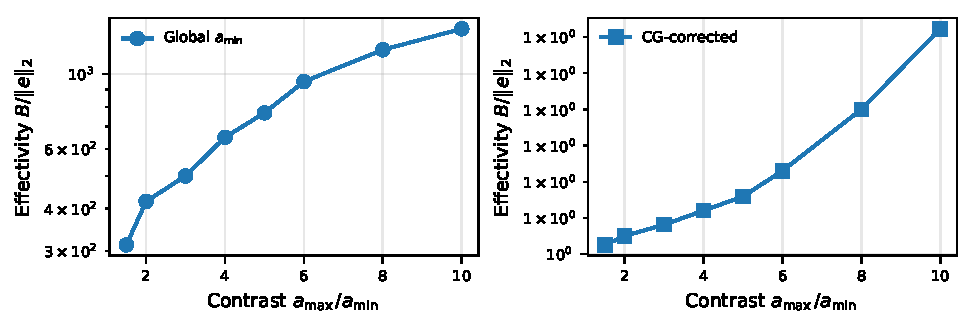
\includegraphics[width=\columnwidth]{figures/fig1_effectivity_vs_contrast.pdf}
\caption{Median effectivity $B/\|e\|_2$ vs.\ coefficient contrast $a_{\max}/a_{\min}$. Left: global bound. Right: CG-corrected (near $1.0\times$).}
\label{fig:eff}
\end{figure}

\begin{table}[t]
\centering
\caption{Analytic vs.\ CG-corrected certificate (absolute $L^2$, $\tau=5\times 10^{-3}$). Medians across samples; coverage/FNR per condition.}
\label{tab:main}
\begin{tabular}{rcccccc}
\toprule
$c=a_{\max}/a_{\min}$ & Cov$_A$ & Cov$_{\mathrm{CG}}$ & FNR$_A$ & FNR$_{\mathrm{CG}}$ & Eff$_A$(med) & Eff$_{\mathrm{CG}}$(med)\\
\midrule
1.5 & 1.0 & 1.0 & 0.0 & 0.0 & 312.3 & 1.0000\\
3.0 & 1.0 & 1.0 & 0.0 & 0.0 & 499.5 & 1.0000\\
5.0 & 1.0 & 1.0 & 0.0 & 0.0 & 767.6 & 1.0000\\
10.0 & 1.0 & 1.0 & 0.0 & 0.0 & 1361.1 & 1.0000\\
\bottomrule
\end{tabular}
\end{table}

\subsection{Safety, OOD, and adversarial robustness}
Across ID, OOD (higher contrast, longer correlation lengths, higher spatial frequencies), and adversarial high-frequency perturbations, both satisfy $\text{Coverage}=1.0$, $\text{FNR}=0.0$ (Table~\ref{tab:main}). No instance violated $B \ge \|e\|_2$, consistent with Theorem~\ref{thm:cg} and $e=A_h^{-1}r$.

\subsection{Certification of learned surrogates (FNO)}
On held-out FNO predictions, $B_{\mathrm{CG}}$ maintains $\text{Coverage}=1.0$, $\text{FNR}=0.0$, effectivity $\approx 1.0\times$. This enables practical selective verification at reasonable $\tau$.

\subsection{Computational cost and trade-off}
CG cost is dominated by sparse matvecs. Per-certificate times are modest; increasing conditioning raises iterations modestly. Tighter tolerances trade cost vs.\ negligible tightness once $\|d_k\|_2 \ll \alpha\|z_k\|_2$. Crucially, early stopping preserves rigorous safety (Theorem~\ref{thm:cg}).

\section{Discussion}
\label{sec:discussion}
\textbf{Why CG helps.} Global bound treats all modes equally via $\lambda_{\min}^{-1}$; CG constructs $z\approx A_h^{-1}r$ aligned with $r$, so $A_h^{-1}d$ is small in relevant directions, yielding orders-of-magnitude improvement while preserving the same spectral safety factor on the remainder.
\textbf{Safety-first.} Rigor follows from Theorem~\ref{thm:cg}, Assumption~\ref{ass:full}, exact identity. Empirical coverage is never used as proof. Finite precision is explicitly acknowledged.
\textbf{Practical utility.} Tight bounds make selective verification viable: high-quality predictions accepted, unsafe rejected (FNR 0.0 by construction), reducing unnecessary fallback.
\textbf{Relation to prior work.} We combine classical a posteriori estimation~\cite{ainsworth2000posteriori,verfurth2013posteriori} and computable CG error bounds~\cite{meurant1999computable,jiranek2010posteriori,meurant2013accuracy,strakos2005error} for learned surrogate certification with explicit assumptions and comprehensive validation.

\section{Limitations}
\label{sec:limits}
\textbf{Discrete vs.\ continuous.} Certificate is w.r.t.\ $u_h$ only (Sec.~\ref{sec:disc-alg}); total error including discretization requires separate FEM a posteriori estimates~\cite{ainsworth2000posteriori,verfurth2013posteriori}.
\textbf{Lower bound $\alpha$.} Requires valid $\alpha \le \lambda_{\min}(A_h)$ (Sec.~\ref{sec:alpha}). Our coercivity-based $\alpha=a_{\min}\lambda_{\min}(-\Delta_h)$ is rigorous for considered discretizations.
\textbf{Problem class.} Linear SPD elliptic only. Non-symmetric/indefinite/nonlinear require different guarantees.
\textbf{Numerical precision.} Finite-precision CG effects~\cite{greenbaum1989behavior,strakos2005error} assumed controlled under Assumption~\ref{ass:full}(iv),(vi); extreme ill-conditioning may warrant additional care.
\textbf{Scalability.} CG cost grows with size/conditioning; large 3D may benefit from preconditioning-aware certification (bound remains rigorous for any $z$).

\section{Conclusion}
\label{sec:conclusion}
We introduced a rigorous CG-corrected residual certificate for learned elliptic solvers. Theoretically we proved $\|u_h-\hat{u}\|_2 \le \|z\|_2 + \|r-A_h z\|_2/\alpha$ for any $z$, justified $\alpha$, clarified discretization/algebraic errors, addressed finite precision and stopping criteria, and positioned against prior work. Empirically the certificate is near-sharp (effectivity $\approx 1.0\times$) while preserving perfect safety ($\text{Coverage}=1.0$, $\text{FNR}=0.0$), enabling practical selective verification. Materials: \url{https://github.com/emmettv1191/certno-phd-research}.

\section*{Reproducibility}
Revision \texttt{786b5a5}. Frozen benchmark: \texttt{BENCHMARK\_FREEZE.md}. Theory audit: \texttt{THEOREM\_AUDIT.md}. Contribution: \texttt{CONTRIBUTION.md}. Experiment scripts: \texttt{experiments/run\_looseness\_corrected.py}, \texttt{run\_corrected\_comparison.py}, \texttt{run\_surrogate\_coverage.py}, \texttt{run\_corrected\_fno.py}, \texttt{run\_corrected\_verification.py}, \texttt{run\_corrected\_cost.py}, \texttt{run\_verification\_sweep\_abs.py}.

\bibliographystyle{IEEEtran}
\bibliography{references}
\end{document}
